\documentclass[main]{subfiles}

\begin{document}

\chapter{Post Assembly} 

\section{\knot} \label{section:postassembly:knot}
% historique

\begin{figure}[ht]
    \subfloat[][A synthetic metagenome of 5 species wis a different coverage]{
        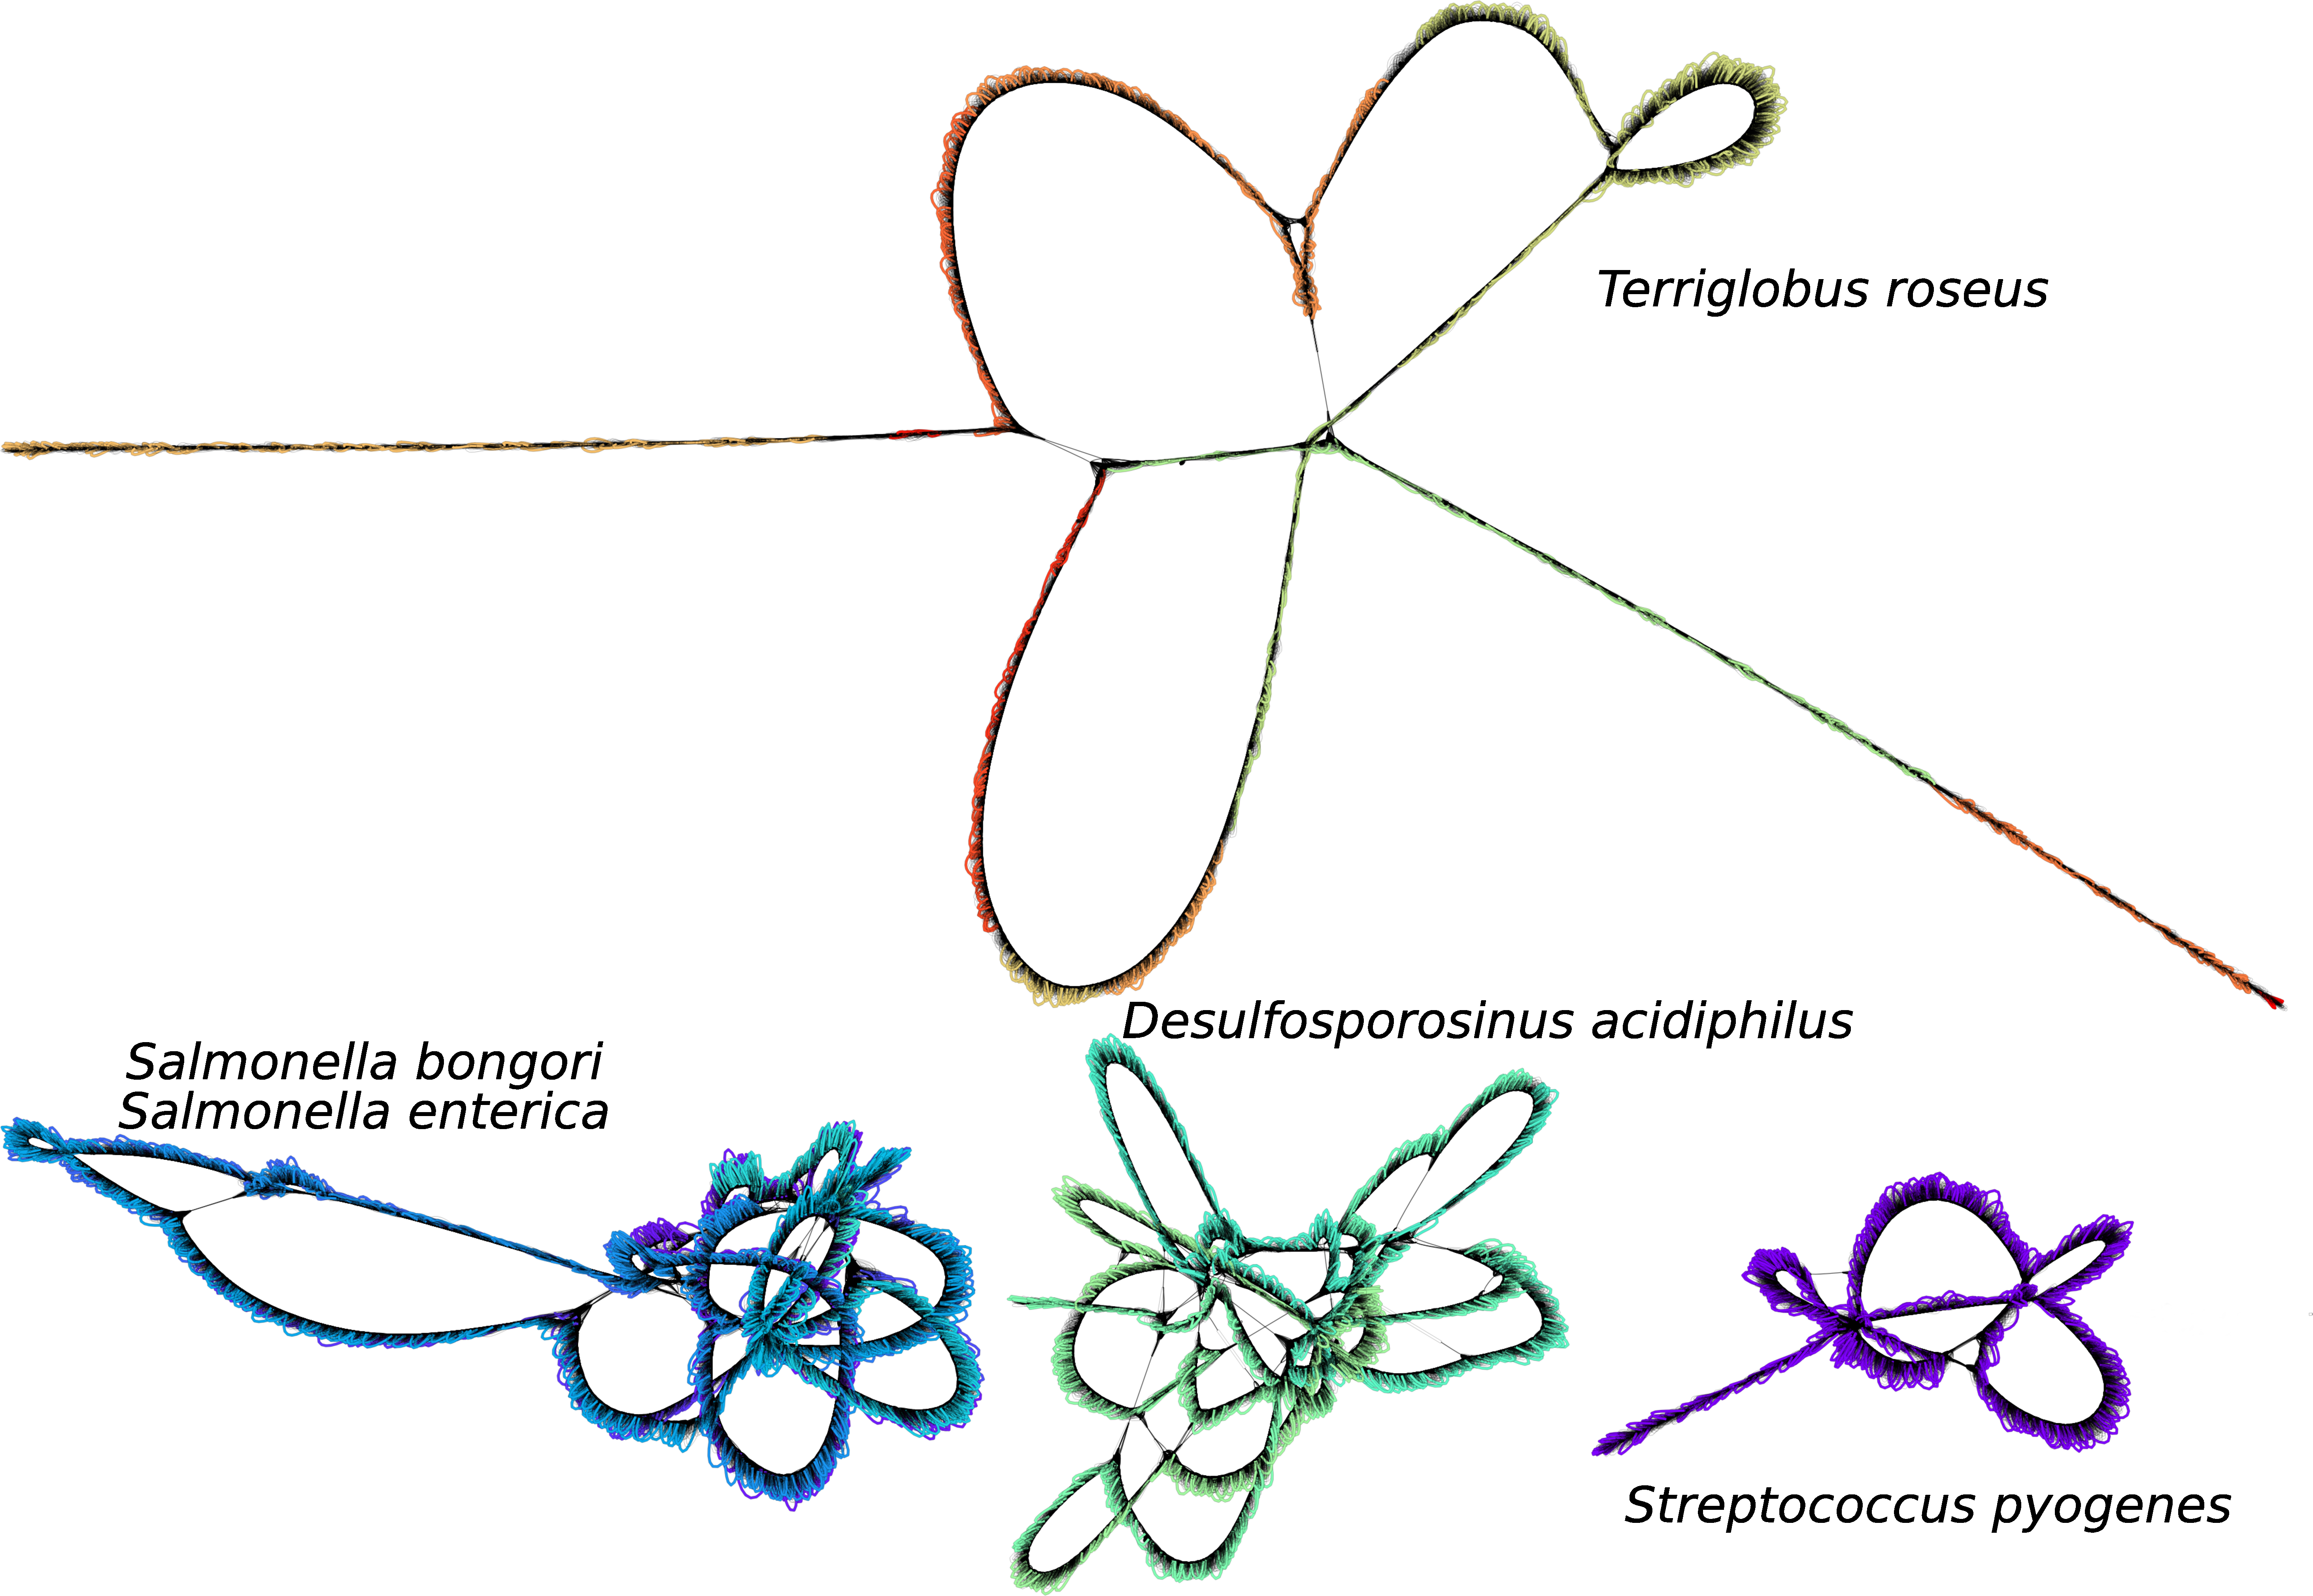
\includegraphics[width=0.9\textwidth]{./postassembly/images/mbrac5_projection.pdf}
        \label{postassembly:fig:intro:mbrac5}
    }
    \newline
    \subfloat[][\textit{Terriglobus roseus} with a 20x coverage]{
        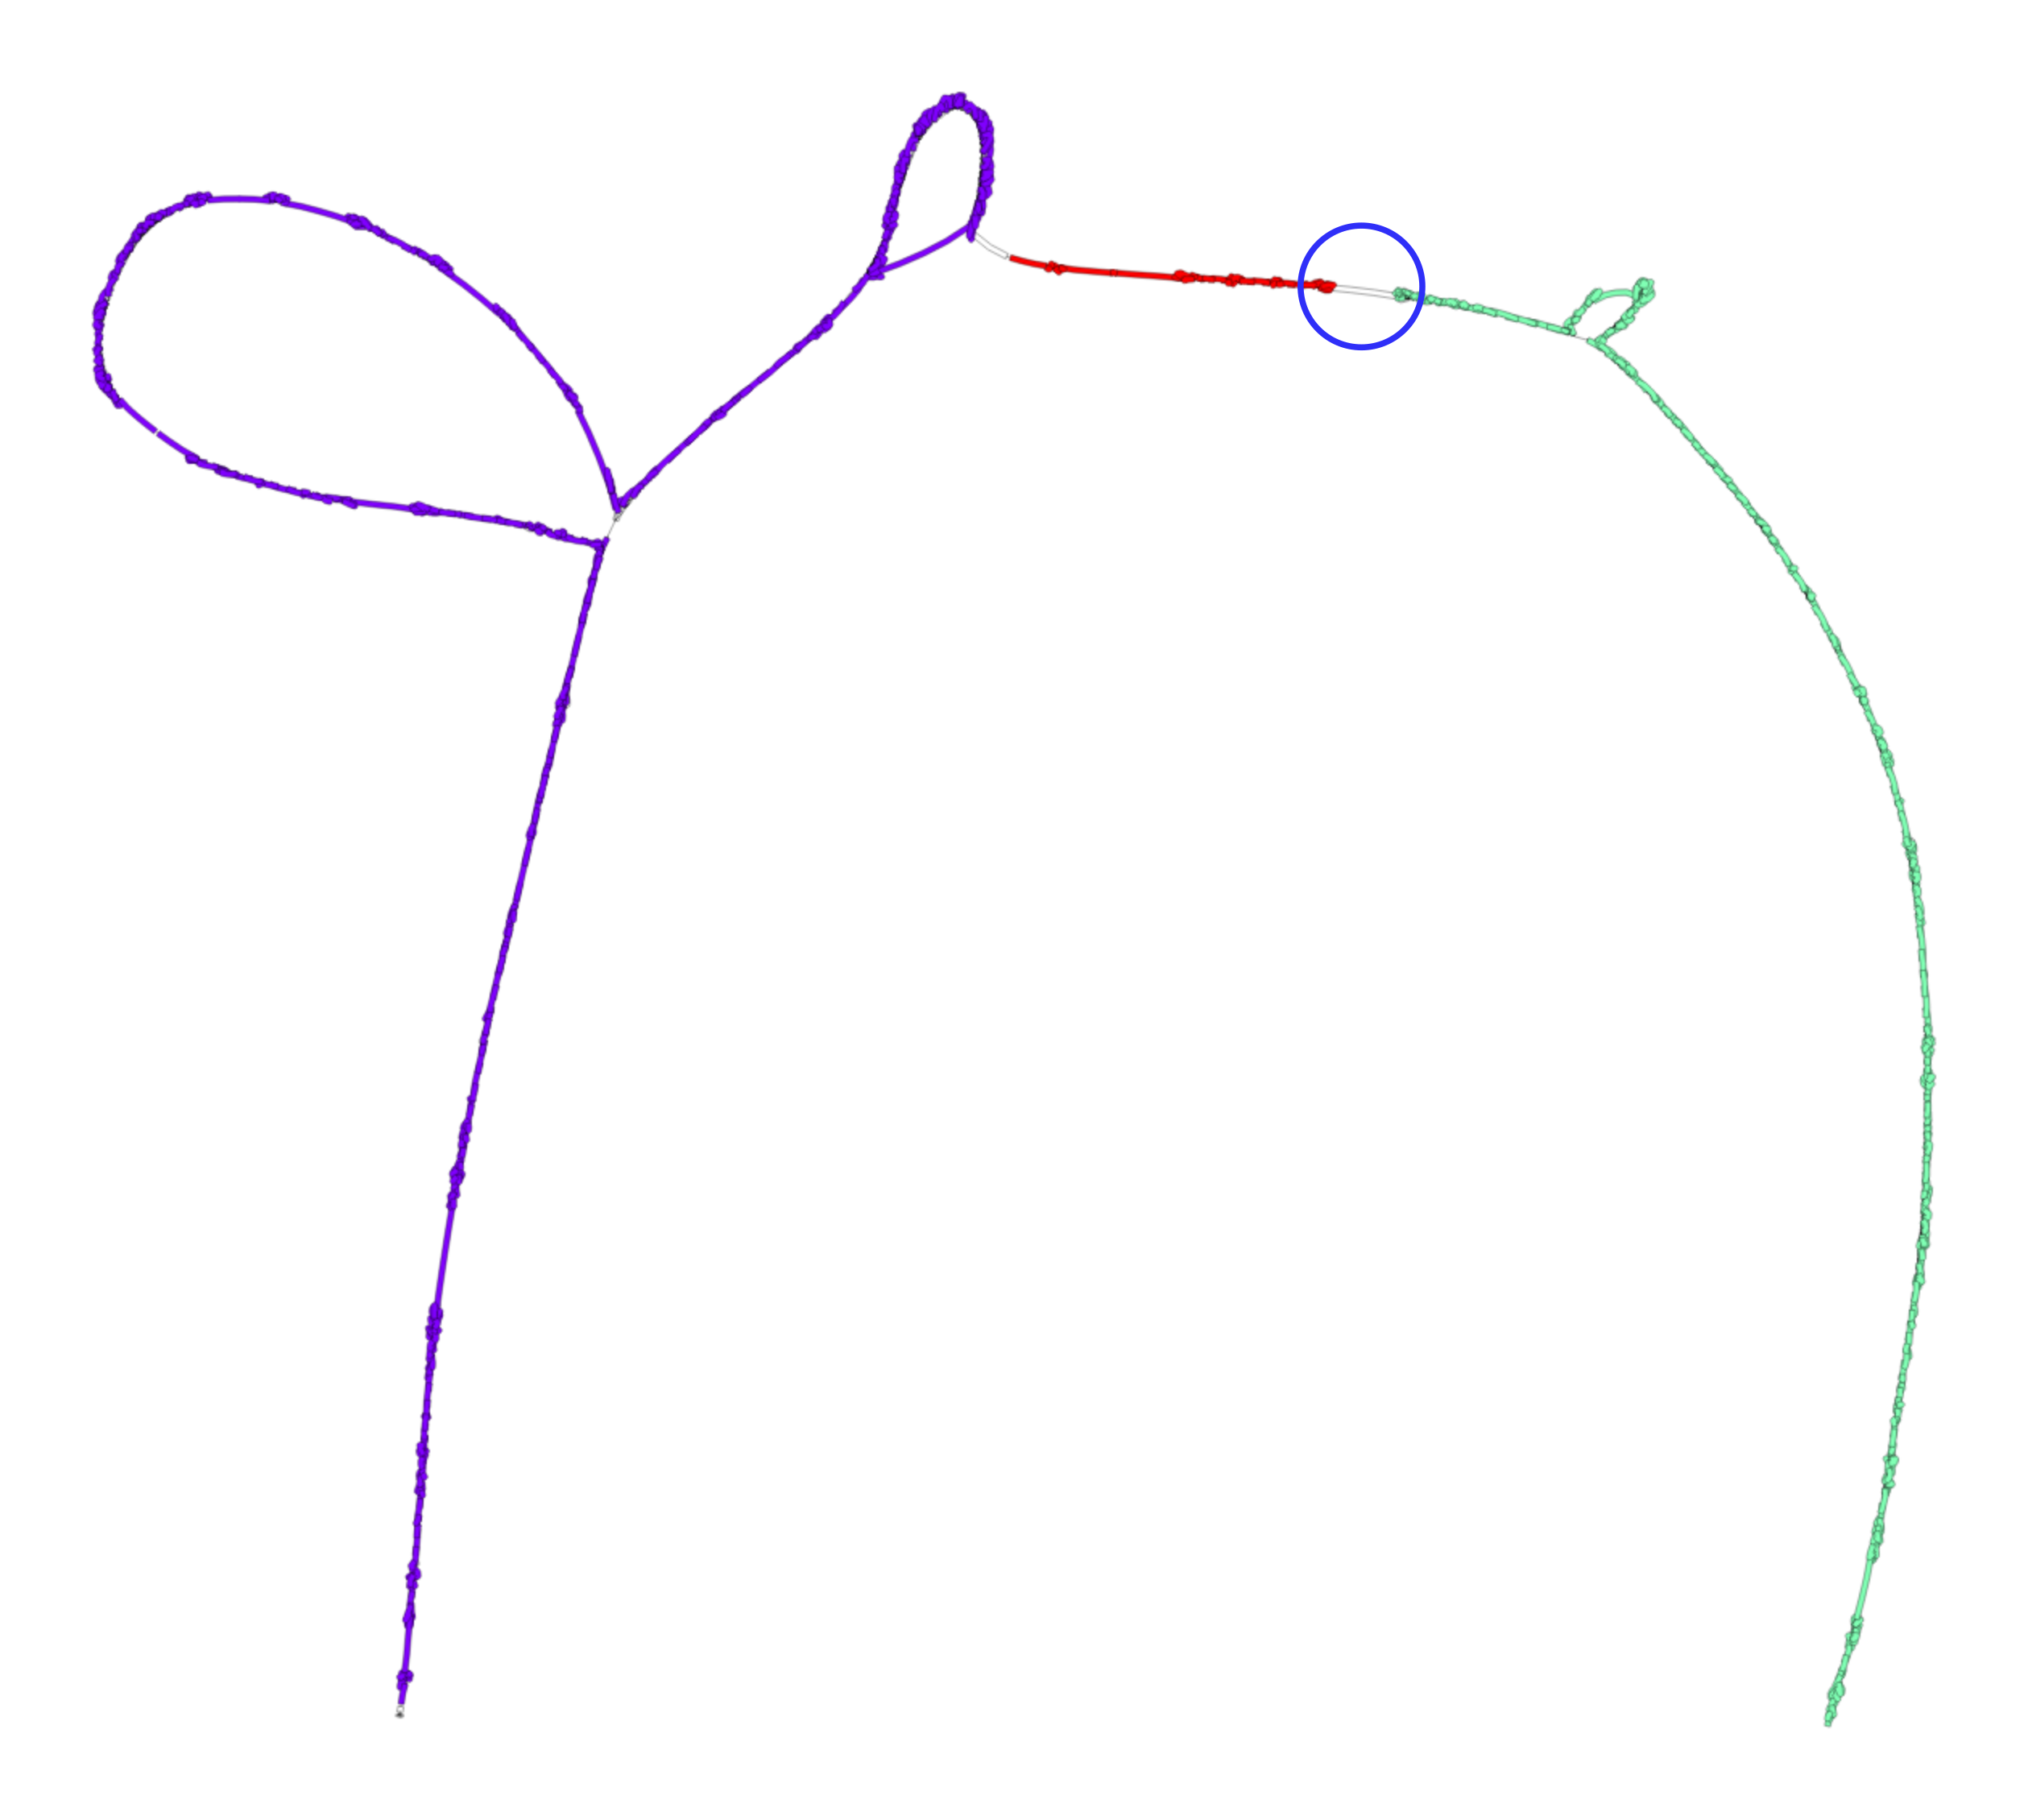
\includegraphics[width=0.9\textwidth]{postassembly/images/t_roseus_projection.png}
        \label{postassembly:fig:intro:troseus}
    }
    \caption{This graph was the overlap graph (found by \minimap), read used by \canu to build a contigs was are colored with same color. We can observe many unexpected fragmentation in (a) and this fragmentation is still be present in genomic context (b)}
    \label{fig:my_label}
\end{figure}

we can cite AMOSvalidate \cite{amosvalidate}, REAPR \cite{REAPR}, FRCbam \cite{FRCbam}, Pilon \cite{Pilon}, VALET \cite{VALET}.
We can evaluate the assembly completeness without genome reference with presence or absence of core genes with BUSCO \cite{busco} or CheckM \cite{checkm}.

\subfile{paper/knot.tex}
%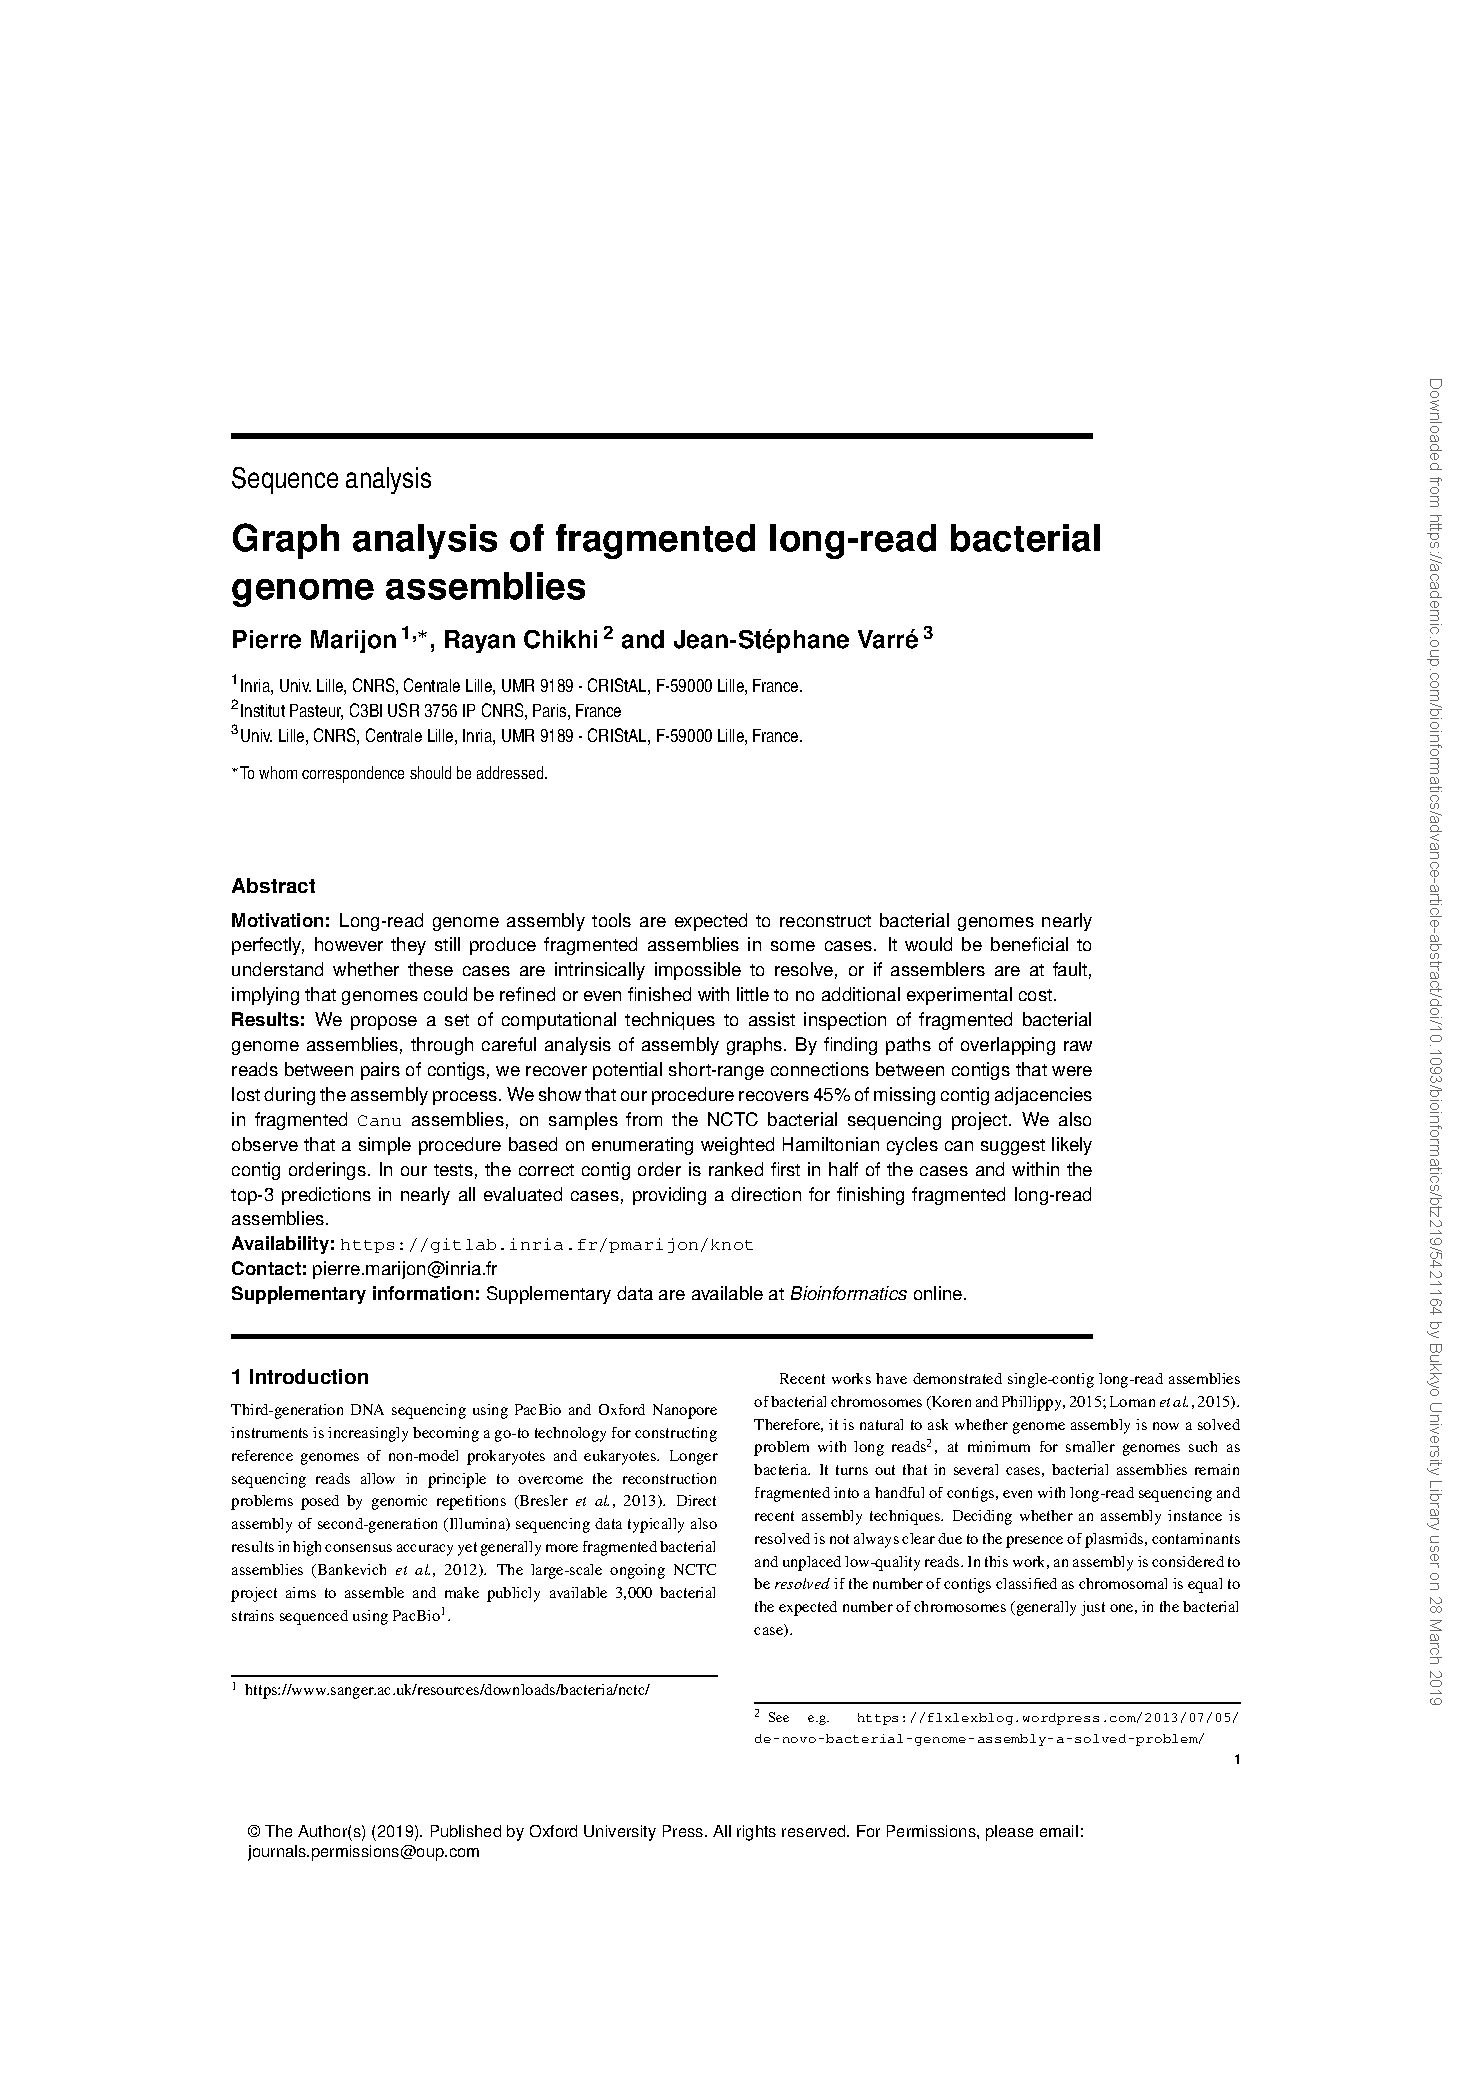
\includepdf[pages=-]{paper/knot.pdf}

\onlyinsubfile{
\bibliographystyle{plainnat}
\bibliography{main}
\addcontentsline{toc}{chapter}{Bibliography}
}



\end{document}